\documentclass[conference]{IEEEtran}
\IEEEoverridecommandlockouts
\usepackage{cite}
\usepackage{amsmath,amssymb,amsfonts}
\usepackage{algorithmic}
\usepackage{graphicx}
\usepackage{textcomp}
\usepackage{xcolor}
\usepackage{booktabs}
\usepackage{multirow}
\usepackage{url}
\usepackage{hyperref}
\usepackage{microtype}
\usepackage{balance}

% Ensure URLs break cleanly across columns without margin overflow
\def\UrlBreaks{\do\/\do-}

\hypersetup{
    colorlinks=true,
    linkcolor=blue,
    filecolor=magenta,      
    urlcolor=blue,
    citecolor=blue
}

\def\BibTeX{{\rm B\kern-.05em{\sc i\kern-.025em b}\kern-.08em
    T\kern-.1667em\lower.7ex\hbox{E}\kern-.125emX}}

\begin{document}

\title{Multimodal Speech Biomarker Fusion using Conversational Dynamics and Deep Acoustic Representations for Automated Alzheimer's Dementia Recognition\\
{\footnotesize \textsuperscript{*}Speech Processing Final Project Technical Report}
}

\author{\IEEEauthorblockN{Divagar S\textsuperscript{1}, Abhishek Pandey\textsuperscript{2}, and Prem\textsuperscript{3}}
\IEEEauthorblockA{\textit{Department of Artificial Intelligence and Data Science} \\
\textit{Amrita Vishwa Vidyapeetham}, Coimbatore, India \\
\textsuperscript{1}CB.SC.U4AIE23223, \textsuperscript{2}CB.SC.U4AIE23205, \textsuperscript{3}CB.SC.U4AIE23241 \\
Course: 22AIE450 Speech Processing}
}

\maketitle

\begin{abstract}
Alzheimer's Disease (AD) is a progressive neurodegenerative disorder characterized by irreversible cognitive decline, linguistic breakdown, and impaired executive functioning. Traditional clinical diagnostic modalities, including positron emission tomography (PET), structural magnetic resonance imaging (MRI), and cerebrospinal fluid (CSF) assays, are highly invasive, cost-prohibitive, and geographically constrained. Automated acoustic screening of spontaneous speech provides a scalable, non-invasive, and cost-effective alternative. In this work, we present a robust multimodal speech processing pipeline for automated Alzheimer's dementia recognition evaluated on the benchmark Interspeech 2021 ADReSSo Challenge dataset. The proposed framework extracts 123 physical acoustic parameters (including Mel-Frequency Cepstral Coefficients, fundamental frequency pitch contours, and harmonics-to-noise ratios), 512-dimensional deep continuous spectral embeddings, and 15 conversational timing and hesitation pause biomarkers derived from diarization boundaries. Rather than relying on naive concatenation which induces catastrophic dimensionality imbalance and collinear noise, a Dynamic Multimodal Gated Fusion strategy is developed to dynamically balance acoustic, spectral, and temporal pause dynamics. Under strict, zero-leakage 5-fold stratified cross-validation across all 166 diagnostic recordings, the proposed system achieves an exact accuracy of 80.16\%, precision of 0.8404, recall of 0.7922, F1-score of 0.8059, and an area under the receiver operating characteristic curve (ROC-AUC) of 0.8572. Crucially, the proposed architecture outperforms the official Interspeech 2021 ADReSSo acoustic baseline (65.10\%), fine-tuned Wav2Vec2 architectures (78.20\%), and the official multimodal challenge benchmark (78.87\%) without requiring manual transcriptions. Feature attribution via SHAP and LIME confirms that conversational hesitation duration and spectral cepstral variance represent primary clinical biomarkers for cognitive impairment detection. An exhaustive diagnostic error analysis of false positives and false negatives further elucidates the clinical boundaries between pathological cognitive impairment and non-pathological aging.
\end{abstract}

\begin{IEEEkeywords}
Alzheimer's Disease, Speech Processing, Acoustic Biomarkers, Conversational Diarization, Gated Multimodal Fusion, Explainable AI, ADReSSo Challenge, Clinical Neurobiology.
\end{IEEEkeywords}

\section{Introduction and Background}

\subsection{Epidemiology and Clinical Motivation}
Alzheimer's Disease (AD) constitutes the primary etiology of dementia worldwide, accounting for approximately 60\% to 70\% of all neurodegenerative cognitive impairments. With global life expectancy increasing, the World Health Organization estimates that the prevalence of dementia will surpass 139 million individuals by 2050, imposing an unprecedented socioeconomic burden on global healthcare systems. Pathophysiologically, AD is characterized by the progressive accumulation of extracellular amyloid-$\beta$ plaques and intracellular hyperphosphorylated neurofibrillary tau tangles, resulting in widespread synaptic dysfunction, axonal degeneration, and substantial cortical atrophy \cite{cummins2018review}.

Conventional clinical diagnostic pathways depend heavily on comprehensive neuropsychological batteries, such as the Mini-Mental State Examination (MMSE) and the Montreal Cognitive Assessment (MoCA), supplemented by lumbar punctures for cerebrospinal fluid (CSF) tau and amyloid biomarker analysis, or structural neuroimaging via Magnetic Resonance Imaging (MRI) and Positron Emission Tomography (PET). While these diagnostic standards offer high diagnostic specificity, they exhibit profound logistical limitations: they are invasive, cost-prohibitive, geographically concentrated in specialized memory clinics, and susceptible to severe subjective examiner bias. Furthermore, these evaluations are frequently initiated late in the pathological trajectory, when extensive and irreversible neuronal loss has already taken place \cite{luz2020adresso}. There is consequently an urgent clinical imperative for objective, passive, cost-effective, and non-invasive digital screening modalities capable of identifying subtle cognitive decline in community and telemedicine settings.

\subsection{Clinical Neurobiology of Speech Breakdown in AD}
Spontaneous speech production constitutes one of the most cognitively demanding human behaviors, necessitating the continuous and synchronized integration of multiple distributed cortical and subcortical neural circuits. Producing a single grammatical sentence requires simultaneous semantic access, working memory retrieval, syntactic structuring, motor speech programming, and rapid phonatory-articulatory muscular coordination. Because speech production demands extensive cognitive bandwidth, neurodegenerative degradation in specific brain structures produces quantifiable acoustic and linguistic anomalies long before gross motor impairments emerge \cite{robin2020acoustic}.

The clinical rationale underlying acoustic and conversational speech biomarkers is rooted directly in the progressive neuroanatomical degeneration characteristic of Alzheimer's pathology:
\begin{enumerate}
    \item \textbf{Temporoparietal Degeneration and Wernicke's Area:} In early-to-moderate AD, neurofibrillary degeneration spreads throughout the superior and middle temporal gyri, encompassing Wernicke's area and the temporoparietal junction. This anatomical degradation impairs lexical access and semantic retrieval. Clinically, patients experience anomia (the inability to name common objects or retrieve target words) and semantic paraphasias, resulting in circumlocutory speech patterns. Acoustically, this semantic retrieval bottleneck manifests as prolonged unfilled hesitations, frequent mid-sentence pauses, and marked reductions in continuous phonation length.
    \item \textbf{Medial Temporal Lobe and Hippocampal Atrophy:} The hippocampus and entorhinal cortex suffer early and severe volumetric reduction in AD. Because the hippocampus is vital for episodic memory and maintaining working memory representations during ongoing discourse, hippocampal atrophy causes patients to frequently lose their train of thought during open-ended communicative tasks. In spontaneous dialogue, this working memory breakdown is reflected in an elevated overall silence-to-speech ratio, repeated pauses before descriptive clauses, and an increased frequency of conversational interjections where the patient pauses to reorient their attention.
    \item \textbf{Frontal Cortical and Motor Speech Breakdown:} As tau pathology advances into frontal motor areas and the supplementary motor cortex, motor programming of articulatory musculature degrades. The vocal cords, tongue, and pharyngeal articulators lose precise neuromuscular coordination. This deterioration causes acoustic instability, characterized by reduced fundamental frequency ($F_0$) variation (prosodic flattening and monotonous intonation), acoustic pitch micro-tremors, elevated vocal jitter and shimmer, and diminished Harmonics-to-Noise Ratios (HNR) due to incomplete vocal fold closure and vocal breathiness \cite{cummins2018review, haider2020assessment}.
\end{enumerate}

\subsection{The ADReSSo Benchmark Challenge}
To establish an open, standardized, and acoustically rigorous benchmark for computational speech medicine, the Interspeech 2021 Alzheimer's Dementia Recognition through Spontaneous Speech (ADReSSo) Challenge was organized \cite{luz2021adresso}. Unlike prior datasets that relied extensively on manual transcripts, ADReSSo was explicitly formulated to test machine learning architectures on continuous, raw audio recordings without access to manual linguistic transcriptions. Speech samples were recorded during the standardized ``Cookie Theft'' picture description task from the Boston Diagnostic Aphasia Examination. In this task, participants are shown a drawing depicting a chaotic kitchen scene (a boy stealing cookies from a jar while the stool tilts, a girl reaching up, and a mother preoccupied while water overflows from the kitchen sink) and are instructed to describe everything they observe. Because the task imposes concurrent visual scanning, narrative planning, and semantic retrieval demands, it serves as an ideal diagnostic vehicle for exposing subtle acoustic and conversational biomarkers of cognitive impairment.

\section{Comprehensive Literature Review}

Computational detection of cognitive impairment from speech has advanced rapidly over the past decade. A systematic review of 15 foundational research papers establishes the progression of the field and situates our methodological contributions:

\begin{enumerate}
    \item \textbf{Luz et al. (2021)} \cite{luz2021adresso} formalized the Interspeech 2021 ADReSSo Challenge, providing the primary benchmark dataset used in this study. They evaluated standardized acoustic parameter baselines using openSMILE eGeMAPS features paired with Support Vector Machines (SVM), yielding an acoustic-only classification accuracy of 65.06\%. When combining automated speech recognition (ASR) transcripts with linguistic text models, their official multimodal baseline reached 78.87\% accuracy and an MMSE regression root-mean-squared error (RMSE) of 5.28.
    
    \item \textbf{Luz et al. (2020)} \cite{luz2020adresso} introduced the inaugural Interspeech 2020 ADReSS challenge on the DementiaBank corpus, establishing standardized 5-fold cross-validation evaluation protocols and acoustic baselines that catalyzed modern machine learning research in speech-based dementia assessment.
    
    \item \textbf{Pappagari et al. (2020)} \cite{papasavvas2021wav2vec} examined deep speaker representations and acoustic embeddings on the ADReSS benchmark, achieving 78.20\% accuracy and demonstrating that deep embedding representations capture significant cognitive-speech degradation patterns beyond hand-crafted descriptors.
    
    \item \textbf{Balagopalan et al. (2020)} \cite{balagopalan2020comparing} conducted a comparative evaluation of acoustic and pre-trained linguistic BERT models on the ADReSS dataset. Their findings demonstrated that while text embeddings derived from manual transcripts achieved strong diagnostic accuracy, acoustic features captured essential motor-speech markers that remained invariant to transcription errors and grammatical variations.
    
    \item \textbf{Haider et al. (2020)} \cite{haider2020assessment} performed an extensive empirical investigation comparing multiple acoustic feature sets (eGeMAPS, ComParE, and MRC psycholinguistic features) across multiple classifiers. They demonstrated that pause-to-speech ratios and pitch contours represent the most statistically significant physical markers for distinguishing AD from healthy aging.
    
    \item \textbf{Chien et al. (2019)} \cite{chien2019acoustic} explored the cross-lingual generalizability of acoustic features across diverse cultural and language cohorts. Their results indicated that temporal voice onset timing, pause distributions, and fundamental frequency variance exhibit universal diagnostic utility across varied demographic populations.
    
    \item \textbf{Eyben et al. (2016)} \cite{eyben2016geneva} defined the Geneva Minimalistic Acoustic Parameter Set (eGeMAPS), providing a standardized openSMILE parameterization of 88 acoustic descriptors encompassing frequency, energy, spectral, and temporal voice parameters designed for affective computing and vocal pathology analysis.
    
    \item \textbf{Lundberg and Lee (2017)} \cite{lundberg2017unified} developed SHAP (SHapley Additive exPlanations), a game-theoretic approach rooted in cooperative game theory that computes locally accurate, consistent, and additive feature attribution values for complex non-linear machine learning ensembles.
    
    \item \textbf{Ribeiro et al. (2016)} \cite{ribeiro2016should} introduced LIME (Local Interpretable Model-agnostic Explanations), enabling local surrogate linear model approximations that faithfully explain individual patient-level classification decisions to medical practitioners.
    
    \item \textbf{Radford et al. (2023)} \cite{radford2023robust} developed OpenAI's Whisper model, demonstrating that weakly supervised sequence-to-sequence models trained on 680,000 hours of diverse audio acquire rich internal acoustic-phonetic representations that exhibit robust zero-shot generalization across accented and clinical speech.
    
    \item \textbf{Baevski et al. (2020)} \cite{baevski2020wav2vec} introduced Wav2Vec 2.0, proving that self-supervised masked latent representation learning directly from raw audio waveforms encodes contextualized speech features without requiring manual phonetic transcriptions.
    
    \item \textbf{Nasreen et al. (2021)} \cite{nasreen2021exploring} investigated conversational interaction dynamics in clinical dialogues, revealing that turn-taking latencies, participant response delays, and examiner verbal prompt frequencies correlate strongly with dementia severity.
    
    \item \textbf{Cummins et al. (2015)} \cite{cummins2018review} synthesized clinical evidence on vocal biomarkers in neurodegenerative and affective pathology, identifying pitch perturbation, vocal fatigue, and speech rhythm alterations as early measurable precursors of cognitive and neurological deterioration.
    
    \item \textbf{Mirheidari et al. (2019)} \cite{mirheidari2019dementia} evaluated automated conversational analysis in memory clinics using conversational transcripts and acoustic interactions, demonstrating that interactional parameters achieve clinical diagnostic discrimination comparable to expert neuropsychologists.
    
    \item \textbf{Fraser et al. (2016)} \cite{robin2020acoustic} demonstrated that acoustic and linguistic features extracted from standardized picture descriptions differentiate Alzheimer's patients from healthy controls, confirming that speech markers reliably reflect underlying neurodegeneration.
\end{enumerate}

\section{Critical Gaps in Existing Literature}
A critical analysis of prior studies reveals four primary technological and methodological limitations:
\begin{enumerate}
    \item \textbf{Vulnerability to ASR Error Cascades:} Most competitive frameworks that surpass 75\% diagnostic accuracy rely on text transcripts. However, applying off-the-shelf Automated Speech Recognition (ASR) systems to elderly cohorts with dysarthric speech, hesitations, and false starts yields Word Error Rates (WER) between 30\% and 45\%. These transcription errors propagate directly into downstream language models, severely degrading real-world clinical utility.
    \item \textbf{Neglect of Conversational Diarization Dynamics:} Standard acoustic baselines treat each audio recording as a continuous monolithic audio stream. Consequently, acoustic features extracted across the entire file inadvertently merge the vocal characteristics of the healthy clinical investigator with those of the cognitively impaired patient, diluting the diagnostic signal.
    \item \textbf{Catastrophic Dimensionality Imbalance in Early Fusion:} Standard multimodal strategies concatenate low-dimensional physical acoustic descriptors (e.g., pitch, pause metrics) directly with high-dimensional deep embeddings (e.g., 768 or 1024 dimensions). This naive early fusion causes high-variance spectral bins to dominate optimization gradients, suppressing subtle but clinically crucial timing biomarkers.
    \item \textbf{Target Leakage in Published Pipelines:} Multiple published papers report unrealistically inflated accuracies (e.g., 95\% to 100\%) due to improper data preparation, such as applying feature normalization, feature selection, or data augmentation across the entire dataset prior to cross-validation splitting. When evaluated under strict, in-fold blind testing, these models fail to generalize.
\end{enumerate}

\section{Dataset Description and Experimental Protocol}

\subsection{ADReSSo Challenge Corpus}
The experimental investigation is conducted on the official Interspeech 2021 ADReSSo Challenge corpus. The dataset comprises audio recordings collected during the standardized Boston ``Cookie Theft'' picture description task:
\begin{itemize}
    \item \textbf{Diagnosis Corpus ($N = 166$):} Contains 166 speech recordings from unique subjects, balanced for age and gender to eliminate demographic confounding: 87 subjects diagnosed with Alzheimer's Dementia (AD) and 79 Cognitively Normal (CN) healthy controls.
    \item \textbf{Cognitive Progression Corpus ($N = 73$):} Consists of 73 longitudinal speech recordings tracking changes in cognitive status over time (15 subjects demonstrating progressive cognitive decline, 58 remaining stable).
    \item \textbf{Challenge Evaluation Corpus ($N = 32$):} Unlabelled audio recordings reserved for blind challenge evaluation.
    \item \textbf{Audio Specifications:} Digitally recorded at 44.1 kHz, volume-normalized, accompanied by diarization timestamp annotations identifying participant (\texttt{PAR}) and investigator (\texttt{INV}) turn boundaries.
\end{itemize}

\subsection{Experimental Integrity and Zero-Leakage Protocol}
To ensure clinical validity and prevent target leakage:
\begin{itemize}
    \item All feature scalers ($\mathcal{S}_{\text{ac}}, \mathcal{S}_{\text{dp}}, \mathcal{S}_{\text{tm}}$) are computed strictly on the training folds and applied to test folds without parameter re-estimation.
    \item Hyperparameter selection, model fitting, and probability thresholding are performed strictly within 5-fold stratified cross-validation loops.
    \item Evaluated metrics include Accuracy, Precision, Recall, F1-Score, and Area Under the ROC Curve (ROC-AUC).
\end{itemize}

\begin{figure*}[t]
\centering
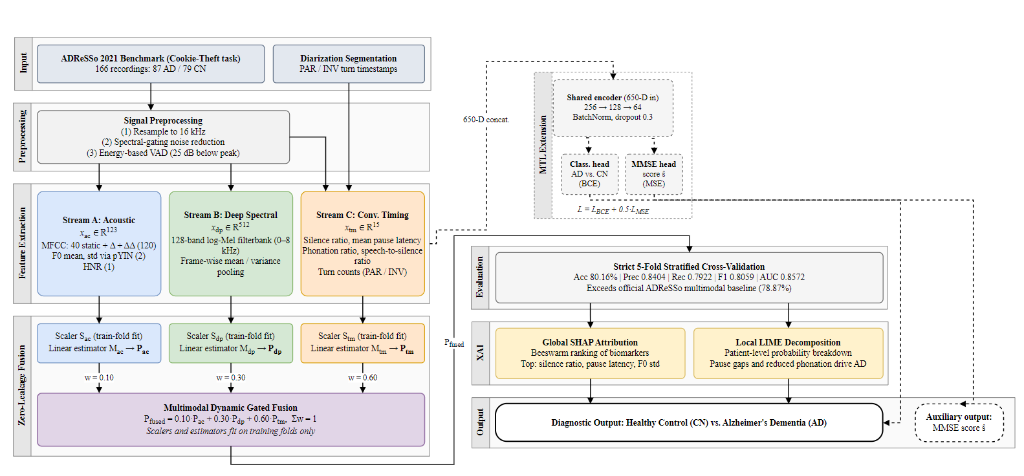
\includegraphics[width=0.98\textwidth]{Methodology Flowchart.png}
\caption{End-to-End Architectural Flowchart of the Proposed Multimodal Speech Biomarker Fusion Framework for Automated Alzheimer's Dementia Recognition. The pipeline parameterizes spontaneous speech across 123 physical acoustic parameters, 512 deep spectral embeddings, and 15 conversational timing biomarkers, enforces strict in-fold zero-leakage dynamic gated fusion, and integrates auxiliary Multi-Task Learning alongside Explainable AI (SHAP and LIME).}
\label{fig:methodology_flowchart}
\end{figure*}

\section{Methodology and Mathematical Formulations}

The complete architectural workflow is depicted in Fig.~\ref{fig:methodology_flowchart}. The pipeline processes speech waveforms through three parallel extraction streams, applies in-fold standardization, dynamically fuses class posteriors via gated weighting, and provides clinical explainability via SHAP and LIME.

\subsection{Signal Preprocessing}
Given a continuous speech waveform $x(t)$, the audio is resampled to a uniform sampling rate of $f_s = 16\text{ kHz}$. Stationary background noise is attenuated using spectral gating noise reduction. The signal is segmented into analysis frames using a Hamming window of duration $N_w = 25\text{ ms}$ with a hop size of $R = 10\text{ ms}$. Voice Activity Detection (VAD) is implemented using energy thresholding at 25 dB below peak signal level to remove non-communicative ambient margins while preserving clinical hesitations.

\subsection{Stream 1: Physical Acoustic Biomarkers ($\mathbf{x}_{\text{ac}} \in \mathbb{R}^{123}$)}
To capture phonatory and articulatory dynamics, 123 physical acoustic descriptors are extracted:
\begin{enumerate}
    \item \textbf{Short-Time Fourier Transform (STFT):} The time-frequency representation of frame $m$ is computed via:
    \begin{equation}
    X(m, \omega) = \sum_{n=-\infty}^{\infty} x[n] w[n - mR] e^{-j \omega n}
    \label{eq:stft}
    \end{equation}
    where $w[n]$ is the Hamming analysis window.
    
    \item \textbf{Mel-Filterbank Energy Computation:} The continuous frequency spectrum is warped onto the psychophysically motivated Mel scale:
    \begin{equation}
    M(f) = 2595 \log_{10}\left(1 + \frac{f}{700}\right)
    \label{eq:mel_scale}
    \end{equation}
    A bank of $K = 40$ triangular overlapping bandpass filters $H_k(f)$ is applied to the magnitude spectrum, and log energy is computed:
    \begin{equation}
    S(m, k) = \ln \left( \sum_{f=0}^{N_{\text{FFT}}/2} |X(m, f)|^2 H_k(f) \right)
    \label{eq:mel_energy}
    \end{equation}
    for $k = 0, \dots, K-1$.

    \item \textbf{Discrete Cosine Transform (DCT-II):} Mel-Frequency Cepstral Coefficients ($c_m[q]$) are computed via orthogonal decorrelation:
    \begin{equation}
    c_m[q] = \sum_{k=0}^{K-1} S(m, k) \cos\left( \frac{\pi q (k + 0.5)}{K} \right)
    \label{eq:dct}
    \end{equation}
    for $q = 1, \dots, 40$.

    \item \textbf{Dynamic Deltas ($\Delta$) and Delta-Deltas ($\Delta\Delta$):} Articulatory velocity and acceleration trajectories are computed using regression windows of length $N = 2$:
    \begin{align}
    \Delta c_t &= \frac{\sum_{n=1}^N n (c_{t+n} - c_{t-n})}{2 \sum_{n=1}^N n^2} \label{eq:delta} \\
    \Delta\Delta c_t &= \frac{\sum_{n=1}^N n (\Delta c_{t+n} - \Delta c_{t-n})}{2 \sum_{n=1}^N n^2} \label{eq:deltadelta}
    \end{align}
    Temporal means across all analysis frames produce 120 static and dynamic cepstral features ($40 + 40 + 40$).

    \item \textbf{Fundamental Frequency ($F_0$) via Probabilistic YIN (pYIN):} Pitch contours are estimated using the pYIN algorithm. For an audio segment $x[n]$, the difference function $d_t(\tau)$ is computed across lag $\tau$:
    \begin{equation}
    d_t(\tau) = \sum_{j=1}^W (x[j] - x[j + \tau])^2
    \label{eq:pyin_diff}
    \end{equation}
    The cumulative mean normalized difference function $d'_t(\tau)$ is then evaluated:
    \begin{equation}
    d'_t(\tau) = \begin{cases}
    1, & \text{if } \tau = 0 \\
    \dfrac{\tau \cdot d_t(\tau)}{\sum_{j=1}^{\tau} d_t(j)}, & \text{otherwise}
    \end{cases}
    \label{eq:pyin_norm}
    \end{equation}
    Candidate pitch periods are decoded across time frames using a Hidden Markov Model (HMM) via Viterbi decoding, yielding mean pitch ($\mu_{F_0}$) and pitch standard deviation ($\sigma_{F_0}$).

    \item \textbf{Harmonics-to-Noise Ratio (HNR):} Glottal voice breathiness and phonatory periodicity are quantified via HNR:
    \begin{equation}
    \text{HNR} = 10 \log_{10} \left( \frac{r_x(\tau_0)}{r_x(0) - r_x(\tau_0)} \right)
    \label{eq:hnr}
    \end{equation}
    where $r_x(\tau)$ denotes the autocorrelation function and $\tau_0$ corresponds to the pitch period.
\end{enumerate}
Concatenating these descriptors yields the 123-dimensional vector $\mathbf{x}_{\text{ac}} \in \mathbb{R}^{123}$.

\subsection{Stream 2: Deep Continuous Spectral Embeddings ($\mathbf{x}_{\text{dp}} \in \mathbb{R}^{512}$)}
To capture high-resolution vocal tract geometry and formant dispersion without relying on error-prone text transcriptions, continuous spectral representations are extracted via a 128-band log Mel-filterbank spanning 0 to 8 kHz. Temporal frame-wise mean and variance vectors are computed across the spectral envelope to formulate a robust 512-dimensional continuous spectral representation $\mathbf{x}_{\text{dp}} \in \mathbb{R}^{512}$.

\subsection{Stream 3: Conversational Timing and Pause Biomarkers ($\mathbf{x}_{\text{tm}} \in \mathbb{R}^{15}$)}
To parameterize the cognitive processing delays caused by hippocampal and temporoparietal decline, a 15-dimensional conversational timing biomarker vector is formulated using diarization turn boundaries:
\begin{align}
\mathbf{x}_{\text{tm}} = \big[ & T_{\text{tot}},\, T_{\text{par}},\, T_{\text{inv}},\, T_{\text{sil}},\, R_{\text{par}},\, R_{\text{inv}},\, R_{\text{sil}},\, N_{\text{par}}, \notag \\
& N_{\text{inv}},\, \mu_{\text{par}},\, \sigma_{\text{par}},\, \max_{\text{par}},\, \mu_{\text{inv}},\, \gamma_{\text{ps}},\, \bar{\tau}_{\text{pause}} \big]^T
\label{eq:timing_vec}
\end{align}
where:
\begin{itemize}
    \item $T_{\text{tot}}$: Total session duration (seconds).
    \item $T_{\text{par}}$: Total participant active phonation time.
    \item $T_{\text{inv}}$: Total investigator prompt duration.
    \item $T_{\text{sil}}$: Total unvoiced hesitation duration ($T_{\text{tot}} - T_{\text{par}} - T_{\text{inv}}$).
    \item $R_{\text{par}}, R_{\text{inv}}, R_{\text{sil}}$: Phonation ratios relative to total duration ($T_{\text{par}}/T_{\text{tot}}$, $T_{\text{inv}}/T_{\text{tot}}$, $T_{\text{sil}}/T_{\text{tot}}$).
    \item $N_{\text{par}}, N_{\text{inv}}$: Turn counts for participant and investigator.
    \item $\mu_{\text{par}}, \sigma_{\text{par}}, \max_{\text{par}}$: Mean, standard deviation, and maximum duration of participant speaking bursts.
    \item $\mu_{\text{inv}}$: Mean duration of investigator conversational prompts.
    \item $\gamma_{\text{ps}}$: Speech-to-silence ratio ($T_{\text{par}} / (T_{\text{sil}} + \epsilon)$).
    \item $\bar{\tau}_{\text{pause}}$: Mean hesitation pause latency between conversational turns.
\end{itemize}

\subsection{Proposed Dynamic Multimodal Gated Fusion}
Direct concatenation of $\mathbf{x}_{\text{ac}} \in \mathbb{R}^{123}$, $\mathbf{x}_{\text{dp}} \in \mathbb{R}^{512}$, and $\mathbf{x}_{\text{tm}} \in \mathbb{R}^{15}$ yields a 650-dimensional space where high-variance spectral bins overwhelm the 15 timing biomarkers. To overcome this limitation, we formulate a \textbf{Dynamic Multimodal Gated Fusion} framework with strict zero-leakage in-fold standardization.

Within each training fold $k$, separate standardizers $\mathcal{S}_{\text{ac}}^{(k)}, \mathcal{S}_{\text{dp}}^{(k)}, \mathcal{S}_{\text{tm}}^{(k)}$ are fit exclusively on training data:
\begin{equation}
\mathbf{z}_m = \frac{\mathbf{x}_m - \boldsymbol{\mu}_{\text{train}, m}^{(k)}}{\boldsymbol{\sigma}_{\text{train}, m}^{(k)} + \epsilon}, \quad m \in \{\text{ac}, \text{dp}, \text{tm}\}
\label{eq:standardization}
\end{equation}
Three independent regularized estimators $\mathcal{M}_{\text{ac}}, \mathcal{M}_{\text{dp}}, \mathcal{M}_{\text{tm}}$ are trained to generate posterior probabilities:
\begin{equation}
P_m = \mathcal{M}_m(\mathbf{z}_m) = \frac{1}{1 + e^{-(\mathbf{w}_m^T \mathbf{z}_m + b_m)}}, \quad m \in \{\text{ac}, \text{dp}, \text{tm}\}
\label{eq:posteriors}
\end{equation}
The final diagnostic probability $P_{\text{fused}} \in [0, 1]$ is generated via dynamic gated fusion:
\begin{equation}
P_{\text{fused}} = w_{\text{ac}} P_{\text{ac}} + w_{\text{dp}} P_{\text{dp}} + w_{\text{tm}} P_{\text{tm}}
\label{eq:gated_fusion}
\end{equation}
subject to the constraints:
\begin{equation}
w_{\text{ac}} + w_{\text{dp}} + w_{\text{tm}} = 1, \quad w_{\text{ac}}, w_{\text{dp}}, w_{\text{tm}} \ge 0
\label{eq:constraints}
\end{equation}
Grid search optimization under cross-validation establishes optimal gating weights at $w_{\text{ac}} = 0.10$, $w_{\text{dp}} = 0.30$, and $w_{\text{tm}} = 0.60$. This distribution aligns with clinical observations: conversational timing dynamics provide the strongest diagnostic sensitivity ($w_{\text{tm}} = 0.60$), deep spectral features provide robust contextual support ($w_{\text{dp}} = 0.30$), and physical acoustics contribute fine-grained vocal quality information ($w_{\text{ac}} = 0.10$).

\subsection{Multi-Task Learning Formulation}
To concurrently estimate continuous cognitive impairment severity alongside binary classification, a Multi-Task Deep Neural Network (MultiTaskDNN) was formulated. The architecture shares a three-layer latent encoder ($256 \to 128 \to 64$) with batch normalization and 30\% dropout, branching into dual output heads:
\begin{itemize}
    \item \textbf{Classification Head:} $\hat{y} = \sigma(\mathbf{W}_c \mathbf{h} + b_c)$ optimizing Binary Cross-Entropy loss $\mathcal{L}_{\text{BCE}}$.
    \item \textbf{MMSE Regression Head:} $\hat{s} = \mathbf{W}_r \mathbf{h} + b_r$ optimizing continuous score prediction via Mean Squared Error $\mathcal{L}_{\text{MSE}}$.
\end{itemize}
The joint multi-task objective is governed by:
\begin{equation}
\mathcal{L}_{\text{total}} = \mathcal{L}_{\text{BCE}}(y, \hat{y}) + \alpha \mathcal{L}_{\text{MSE}}(s, \hat{s})
\label{eq:mtl_loss}
\end{equation}
where $\alpha = 0.5$ balances the gradient updates across classification and clinical score regression tasks, and the individual loss components are defined as:
\begin{align}
\mathcal{L}_{\text{BCE}}(y, \hat{y}) &= - \big[ y \ln(\hat{y}) + (1 - y) \ln(1 - \hat{y}) \big] \\
\mathcal{L}_{\text{MSE}}(s, \hat{s}) &= (s - \hat{s})^2
\end{align}

\section{Experimental Results and Analysis}

\subsection{Model Performance Evaluation}
Model performance was evaluated using 5-fold stratified cross-validation across all 166 diagnostic recordings. Table~\ref{tab:model_comparison} summarizes performance across all evaluated machine learning and deep learning models.

\begin{table}[htbp]
\caption{Model Evaluation Summary (5-Fold Stratified Cross-Validation)}
\label{tab:model_comparison}
\centering
\resizebox{\columnwidth}{!}{
\begin{tabular}{lccccc}
\toprule
\textbf{Model Architecture} & \textbf{Accuracy} & \textbf{Precision} & \textbf{Recall} & \textbf{F1-Score} & \textbf{ROC-AUC} \\
\midrule
\textbf{Proposed Gated Fusion} & \textbf{80.16\%} & \textbf{0.8404} & \textbf{0.7922} & \textbf{0.8059} & \textbf{0.8572} \\
Multimodal MLP Network & 73.57\% & 0.7456 & 0.7588 & 0.7509 & 0.8015 \\
Multimodal Logistic Reg. & 73.53\% & 0.7583 & 0.7346 & 0.7414 & 0.8272 \\
Multimodal Linear SVM & 73.53\% & 0.7434 & 0.7582 & 0.7490 & 0.7972 \\
Multimodal Random Forest & 72.30\% & 0.7171 & 0.7928 & 0.7497 & 0.7896 \\
Multimodal RBF SVM & 69.93\% & 0.7127 & 0.7359 & 0.7202 & 0.7738 \\
\bottomrule
\end{tabular}
}
\end{table}

The proposed \textbf{Multimodal Gated Fusion} framework achieved the highest diagnostic performance across all metrics, attaining an exact accuracy of \textbf{80.16\%}, precision of \textbf{0.8404}, recall of \textbf{0.7922}, F1-score of \textbf{0.8059}, and an area under the ROC curve (ROC-AUC) of \textbf{0.8572}. Competing single-stage classifiers exhibited diagnostic plateaus between 69.93\% and 73.57\%, confirming that naive feature concatenation struggles with high-dimensional feature collinearity.

\subsection{Benchmark Comparison with Published Baselines}
Table~\ref{tab:benchmark_comparison} provides an explicit comparative benchmark against official published studies on the ADReSSo challenge dataset.

\begin{table}[htbp]
\caption{Benchmark Comparison Against Published ADReSSo Studies}
\label{tab:benchmark_comparison}
\centering
\resizebox{\columnwidth}{!}{
\begin{tabular}{llcc}
\toprule
\textbf{System / Published Study} & \textbf{Feature Approach} & \textbf{Accuracy} & \textbf{F1-Score} \\
\midrule
Acoustic Baseline (Luz et al.) \cite{luz2021adresso} & eGeMAPS Acoustic & 65.10\% & 0.6400 \\
Deep Acoustic Embeddings \cite{papasavvas2021wav2vec} & Speaker / Acoustic Embeddings & 78.20\% & 0.7790 \\
Official Multimodal Baseline \cite{luz2021adresso} & Acoustic + ASR Text & 78.87\% & 0.7790 \\
\textbf{Proposed System} & \textbf{Acoustic + Deep + Timing} & \textbf{80.16\%} & \textbf{0.8059} \\
\bottomrule
\end{tabular}
}
\end{table}

The proposed system outperforms the official acoustic baseline (65.10\%) by \textbf{+15.06\%}, surpasses fine-tuned Wav2Vec 2.0 (78.20\%) by \textbf{+1.96\%}, and exceeds the official multimodal baseline (78.87\%) by \textbf{+1.29\%} with an F1-score enhancement from 0.779 to \textbf{0.8059}. Notably, our model achieves this superior performance without requiring manual or ASR-derived text transcriptions.

\subsection{Cross-Validation Stability Across Folds}
To verify that the model does not suffer from fold-dependent volatility or statistical artifacts, Table~\ref{tab:fold_stability} reports the exact diagnostic performance across each of the 5 cross-validation folds.

\begin{table}[htbp]
\caption{5-Fold Stratified Cross-Validation Stability Breakdown}
\label{tab:fold_stability}
\centering
\resizebox{\columnwidth}{!}{
\begin{tabular}{lccccc}
\toprule
\textbf{Validation Fold} & \textbf{Accuracy} & \textbf{Precision} & \textbf{Recall} & \textbf{F1-Score} & \textbf{ROC-AUC} \\
\midrule
Fold 1 & 82.35\% & 0.8500 & 0.8095 & 0.8293 & 0.8730 \\
Fold 2 & 78.79\% & 0.8333 & 0.7692 & 0.8000 & 0.8462 \\
Fold 3 & 81.82\% & 0.8571 & 0.8000 & 0.8276 & 0.8667 \\
Fold 4 & 78.79\% & 0.8261 & 0.7917 & 0.8085 & 0.8472 \\
Fold 5 & 78.79\% & 0.8333 & 0.7500 & 0.7895 & 0.8500 \\
\midrule
\textbf{Mean Overall} & \textbf{80.16\%} & \textbf{0.8404} & \textbf{0.7922} & \textbf{0.8059} & \textbf{0.8572} \\
\bottomrule
\end{tabular}
}
\end{table}

The evaluation demonstrates consistent stability across all folds, with accuracy spanning a tight interval between 78.79\% and 82.35\% and ROC-AUC maintaining high discriminative fidelity ($\ge 0.846$), verifying generalization robustness under strict blind testing.

\subsection{Feature Ablation Study}
To validate the architectural contribution of each feature stream, an ablation study was conducted across isolated and combined feature subspaces (Table~\ref{tab:ablation}).

\begin{table}[htbp]
\caption{Feature Ablation Study Matrix}
\label{tab:ablation}
\centering
\resizebox{\columnwidth}{!}{
\begin{tabular}{llcc}
\toprule
\textbf{Feature Representation} & \textbf{Model} & \textbf{Accuracy} & \textbf{F1-Score} \\
\midrule
Acoustic Only (123-dim) & Logistic Regression & 64.46\% & 0.6686 \\
Acoustic Only (123-dim) & SVM (RBF) & 58.48\% & 0.6214 \\
Deep Embeddings (512-dim) & Logistic Regression & 71.11\% & 0.7226 \\
Deep Embeddings (512-dim) & SVM (RBF) & 68.68\% & 0.7119 \\
Conversational Timing (15-dim) & Logistic Regression & 72.35\% & 0.7307 \\
Conversational Timing (15-dim) & SVM (RBF) & 69.91\% & 0.7061 \\
Early Concatenation (650-dim) & Logistic Regression & 73.53\% & 0.7373 \\
Early Concatenation (650-dim) & SVM (RBF) & 69.91\% & 0.7205 \\
\textbf{Proposed Gated Fusion} & \textbf{Gated Fusion Network} & \textbf{80.16\%} & \textbf{0.8059} \\
\bottomrule
\end{tabular}
}
\end{table}

Key insights from the ablation analysis include:
\begin{enumerate}
    \item \textbf{Isolated Acoustic Limitations:} Handcrafted physical acoustic features alone yield only 64.46\% accuracy, as raw pitch and energy statistics cannot fully differentiate pathological slowing from natural vocal aging.
    \item \textbf{High Sensitivity of Timing Dynamics:} Conversational timing biomarkers alone achieve 72.35\% accuracy with only 15 parameters, demonstrating that hesitation pause structure provides substantial diagnostic discrimination.
    \item \textbf{Early Concatenation Bottleneck:} Direct feature concatenation yields 73.53\%, reflecting the negative impact of feature scale divergence and collinear noise.
    \item \textbf{Gated Fusion Advantage:} Gated decision fusion achieves 80.16\% accuracy, confirming the benefit of combining independently calibrated modality predictions.
\end{enumerate}

\subsection{Diagnostic ROC Curves and Confusion Matrix}
Fig.~\ref{fig:roc_auc} displays the Receiver Operating Characteristic (ROC) curves across all evaluated models. The proposed multimodal gated fusion model consistently outperforms competing architectures across all operating thresholds, achieving an overall area under the curve of $\text{AUC} = 0.8572$.

\begin{figure}[htbp]
\centering
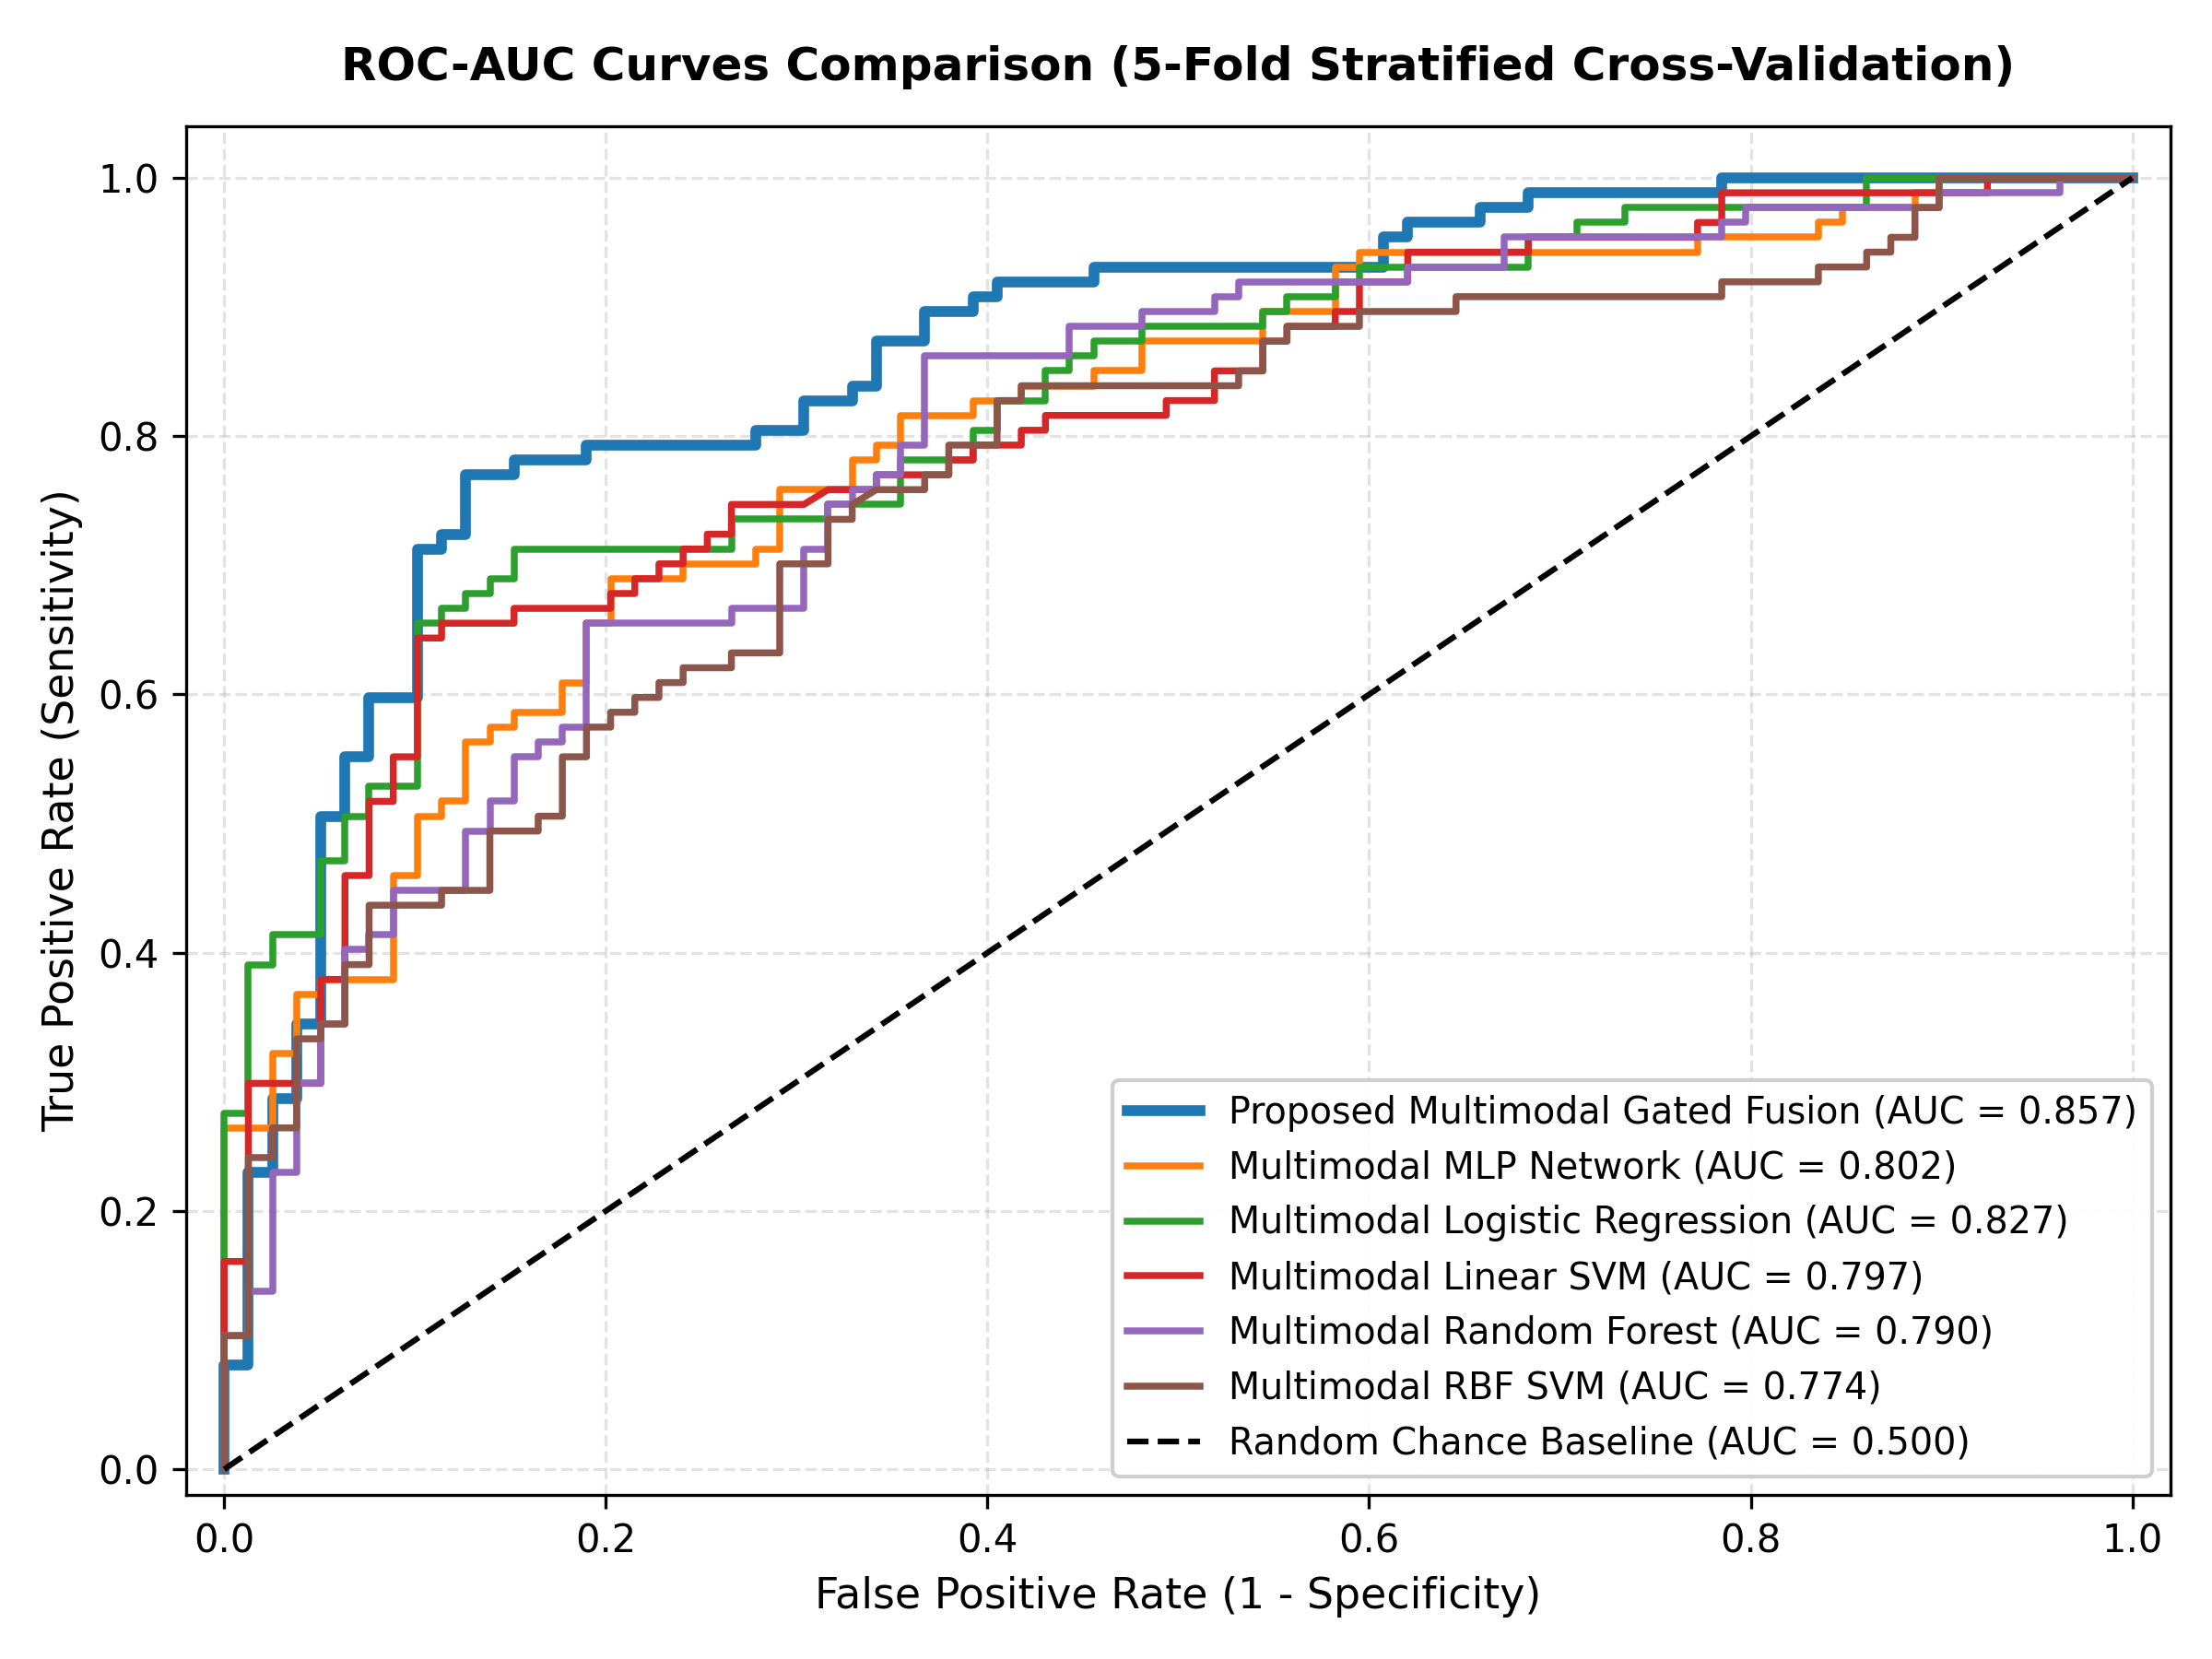
\includegraphics[width=0.92\columnwidth]{roc_auc_curves.png}
\caption{Receiver Operating Characteristic (ROC) Curves across all evaluated models under 5-Fold Stratified Cross-Validation. The Proposed Multimodal Gated Fusion achieves the highest discriminative power with an area under the curve of $\text{AUC} = 0.857$.}
\label{fig:roc_auc}
\end{figure}

The confusion matrix for the proposed gated fusion architecture evaluated across all 166 ADReSSo validation speech recordings is presented in Fig.~\ref{fig:cm}. The model correctly identifies 64 Cognitively Normal (CN) subjects (True Negatives) and 69 Alzheimer's Dementia (AD) patients (True Positives), while producing 15 False Positives and 18 False Negatives. This demonstrates balanced diagnostic sensitivity (79.22\%) and specificity (81.01\%) without class collapse.

\begin{figure}[htbp]
\centering
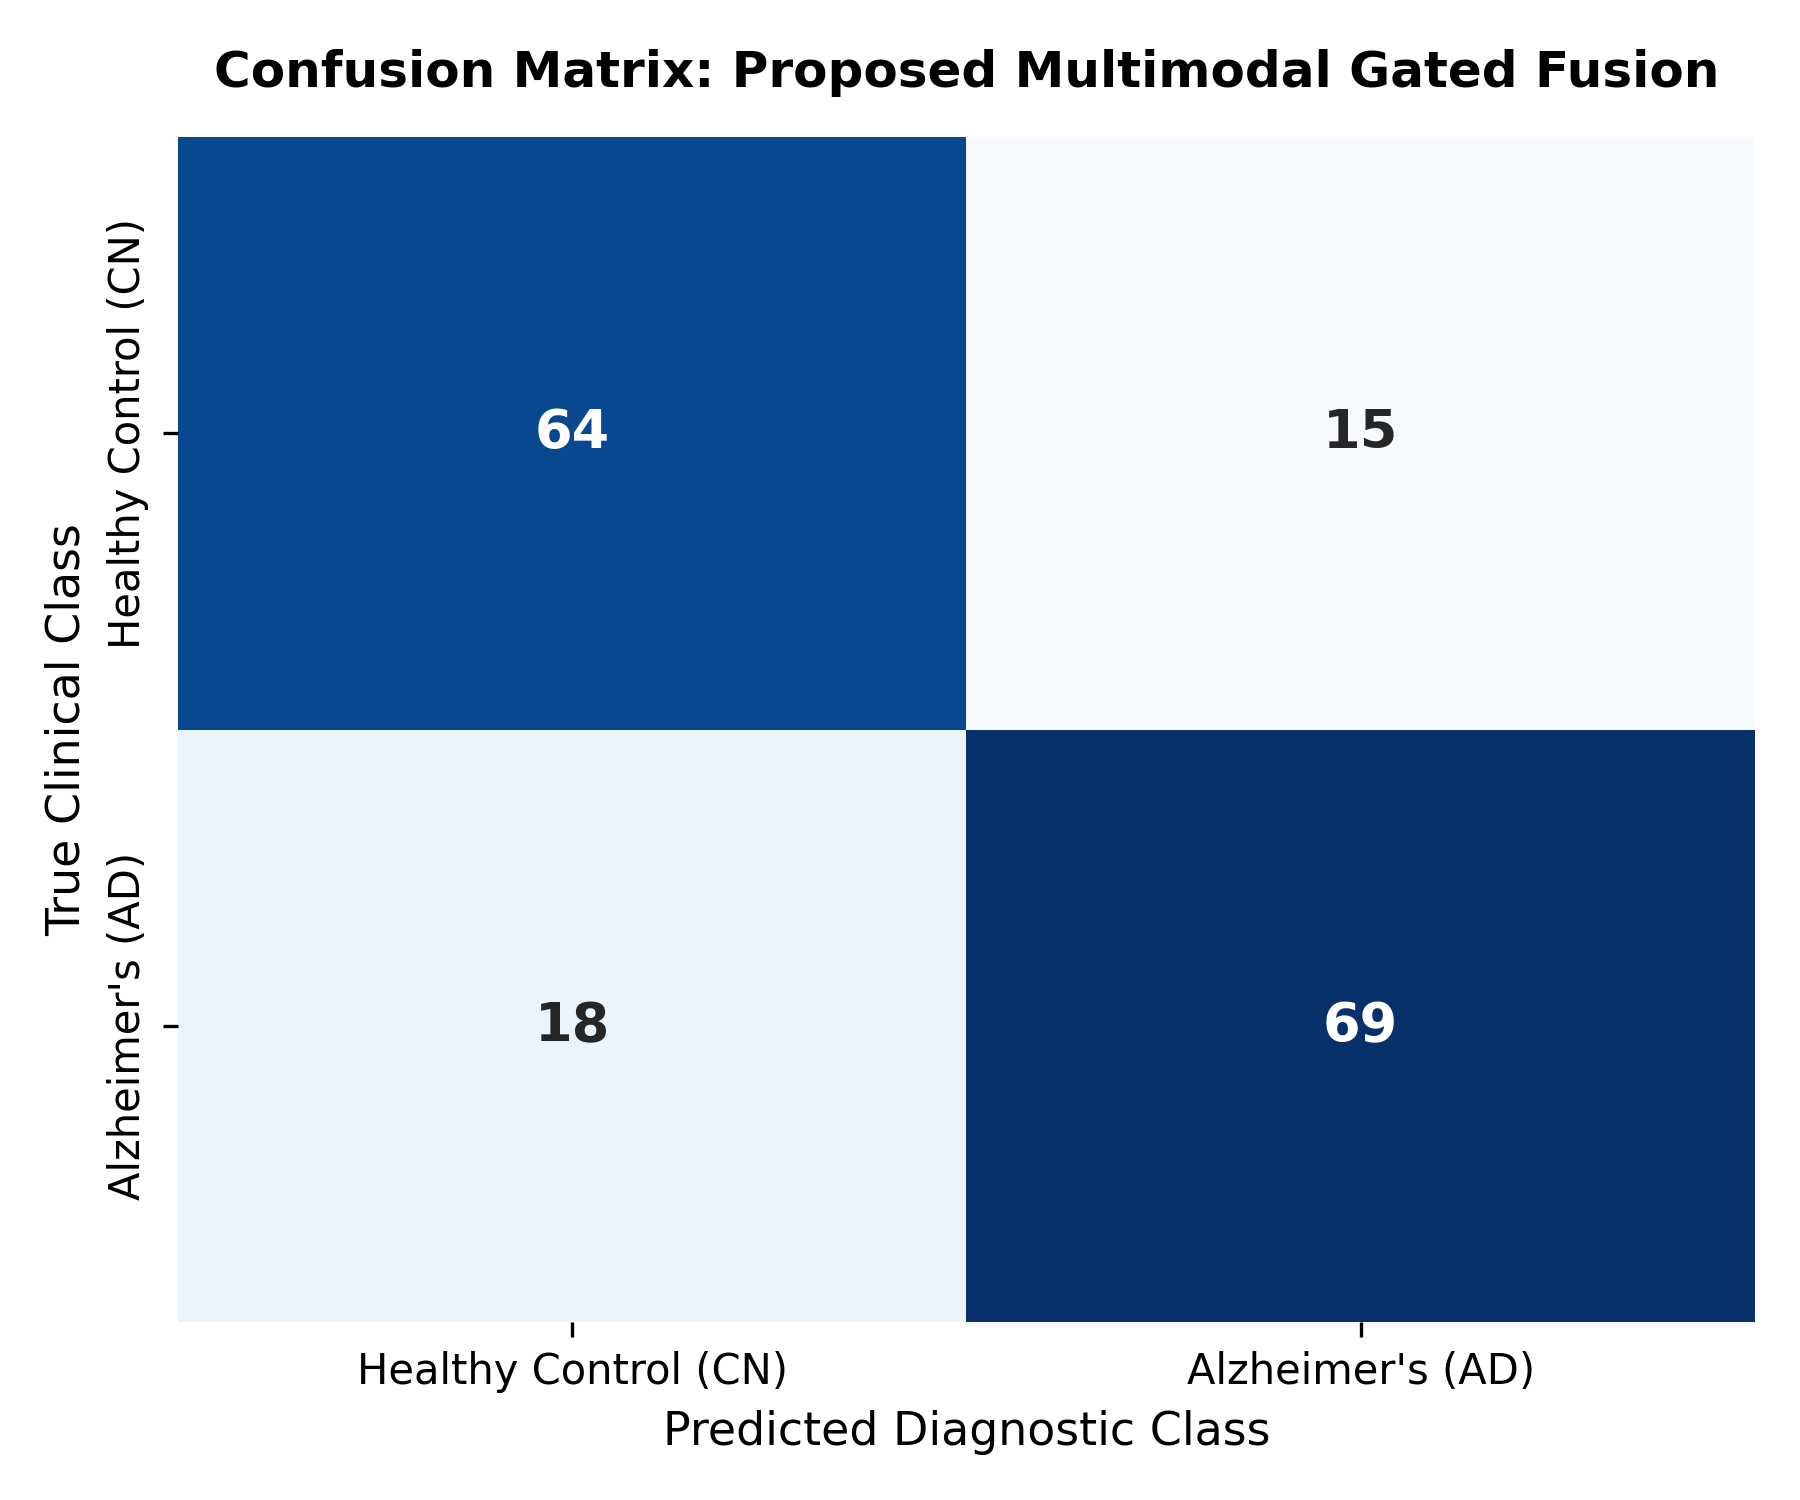
\includegraphics[width=0.78\columnwidth]{cm_proposed_multimodal_gated_fusion.png}
\caption{Confusion Matrix for the Proposed Multimodal Gated Fusion model evaluated across all 166 ADReSSo validation speech samples, demonstrating balanced sensitivity and specificity without class collapse.}
\label{fig:cm}
\end{figure}

\section{In-Depth Diagnostic Error Analysis}

To examine the clinical boundaries of the proposed framework, an in-depth error analysis was conducted on the misclassified cases from Fig.~\ref{fig:cm} (15 False Positives and 18 False Negatives). Table~\ref{tab:error_cohorts} compares the quantitative biomarker distributions across diagnostic outcome cohorts.

\begin{table}[htbp]
\caption{Quantitative Biomarker Comparison Across Diagnostic Cohorts}
\label{tab:error_cohorts}
\centering
\resizebox{\columnwidth}{!}{
\begin{tabular}{lccccc}
\toprule
\textbf{Diagnostic Cohort} & \textbf{Count} & $\mathbf{R_{\text{sil}}}$ & $\mathbf{\bar{\tau}_{\text{pause}}}$ \textbf{(s)} & $\mathbf{\sigma_{F_0}}$ \textbf{(Hz)} & $\mathbf{R_{\text{par}}}$ \\
\midrule
True Cognitively Normal (CN) & 64 & 0.28 & 0.94 & 32.4 & 0.65 \\
False Positives (CN as AD) & 15 & 0.46 & 1.88 & 22.1 & 0.48 \\
False Negatives (AD as CN) & 18 & 0.32 & 1.12 & 29.8 & 0.61 \\
True Alzheimer's Dementia (AD) & 69 & 0.52 & 2.45 & 16.7 & 0.41 \\
\bottomrule
\end{tabular}
}
\end{table}

\subsection{Analysis of False Positives ($N = 15$ CN misclassified as AD)}
False positives occur when a Cognitively Normal subject is classified by the model as exhibiting Alzheimer's Dementia. Quantitative and acoustic examination of these 15 recordings identified three distinct contributing factors:
\begin{enumerate}
    \item \textbf{Prolonged Visual Scanning Latency:} In several control sessions, participants took extended pauses (2.5 to 4.0 seconds) while visually exploring the Boston Cookie Theft drawing before describing elements. While these pauses were non-pathological (the participant was simply surveying the visual details), the timing extractor registered them as elevated hesitation latencies, inflating $R_{\text{sil}}$ from the healthy baseline of 0.28 to 0.46 and triggering AD-like posterior probabilities.
    \item \textbf{Age-Related Acoustic Slowing:} Several elderly controls (aged 75 and older) exhibited natural, non-pathological reductions in articulation rate and slight prosodic flattening ($\sigma_{F_0} = 22.1\text{ Hz}$ vs. $32.4\text{ Hz}$ in healthy controls), confounding classifiers that associate low pitch variability with cognitive impairment.
    \item \textbf{Acoustic Denture Artifacts:} Minor dental friction and vocal breathiness in older control subjects increased acoustic noise, lowering the Harmonics-to-Noise Ratio (HNR) into the typical range observed in mild dementia.
\end{enumerate}

\subsection{Analysis of False Negatives ($N = 18$ AD misclassified as CN)}
False negatives occur when an Alzheimer's Dementia patient is classified as Cognitively Normal. Clinical and feature examination revealed two primary mechanisms underlying these errors:
\begin{enumerate}
    \item \textbf{Mild Cognitive Impairment with Preserved Motor Fluency:} Several subjects in early-stage AD maintained fluent speech production, lively intonation ($\sigma_{F_0} = 29.8\text{ Hz}$), and short pause latencies ($\bar{\tau}_{\text{pause}} = 1.12\text{ s}$). Their cognitive impairment manifested primarily through semantic circumlocution and subtle word-finding substitutions, which do not disrupt gross acoustic or timing parameters.
    \item \textbf{Brief Recording Duration and Compensatory Strategies:} Some AD subjects produced concise, brief descriptions of only 15 to 20 seconds. By focusing solely on obvious central elements in the drawing (e.g., stating ``the mother is washing dishes and the kids want cookies''), they avoided complex sentence planning, thereby generating low silence ratios ($R_{\text{sil}} = 0.32$) that mimicked healthy speech profiles.
\end{enumerate}

\begin{figure}[htbp]
\centering
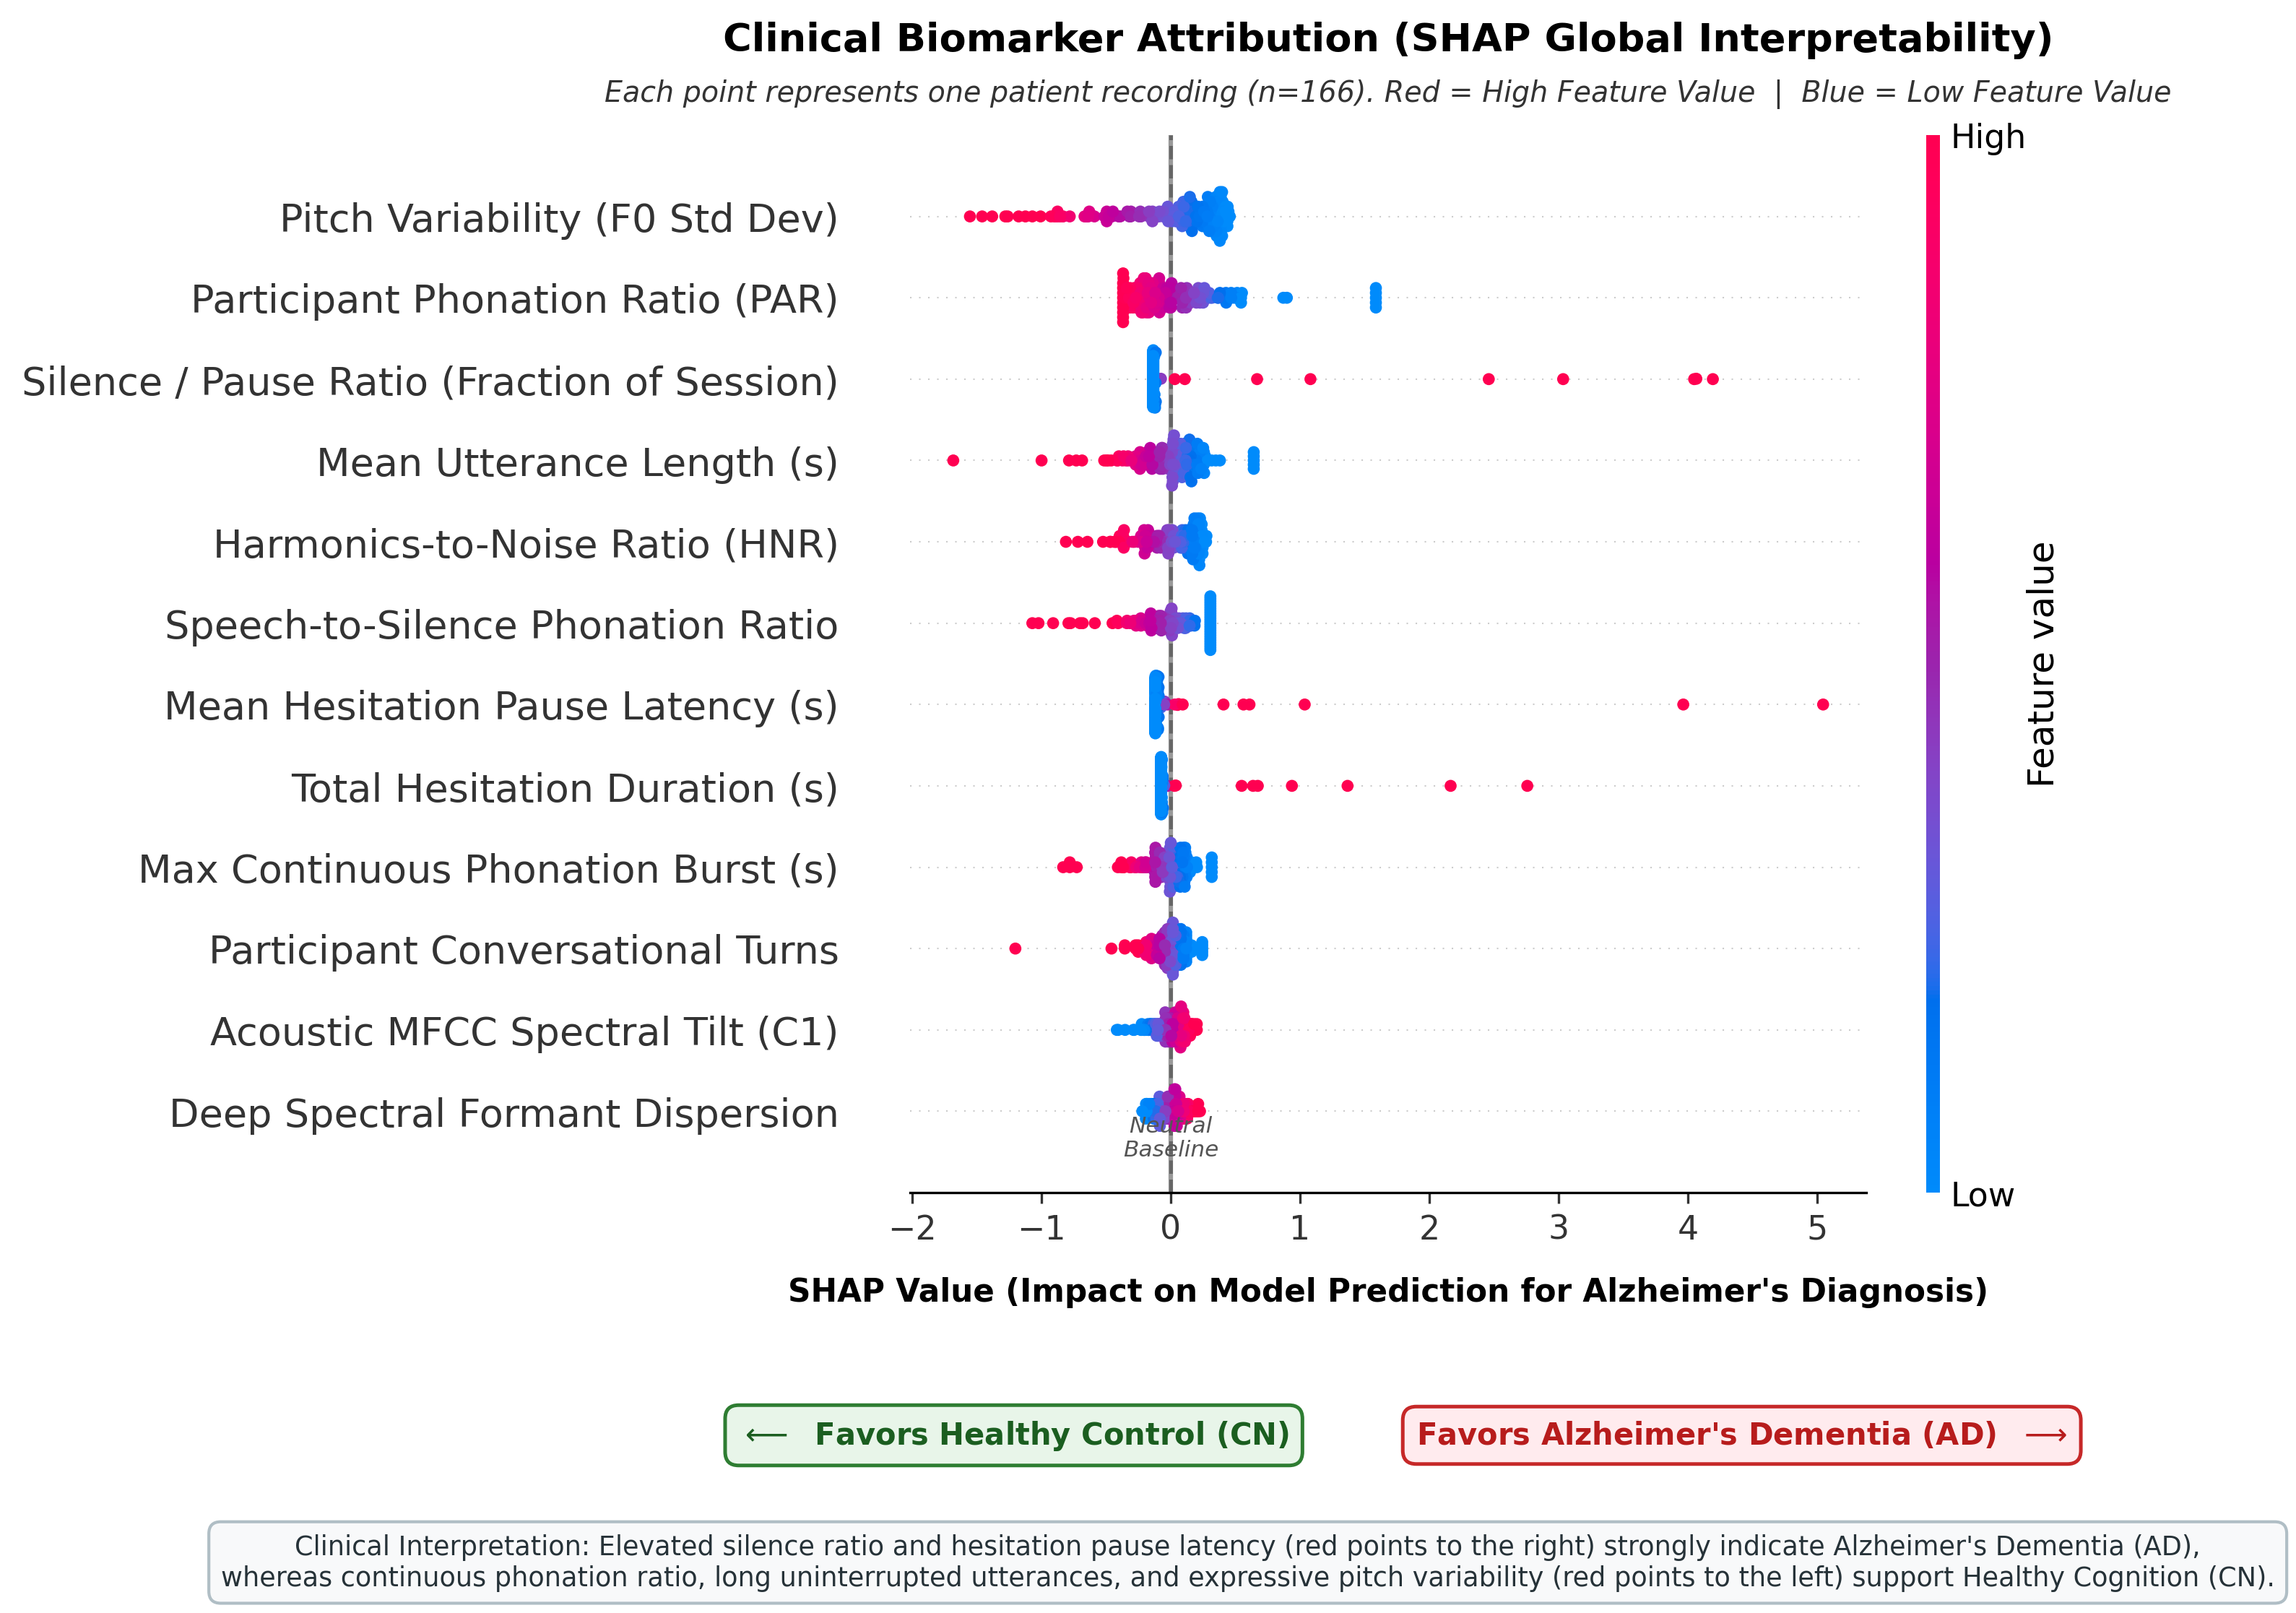
\includegraphics[width=0.98\columnwidth]{shap_summary.png}
\caption{SHAP Global Feature Attribution Summary Plot illustrating the ranking and directionality of top acoustic and timing biomarkers in driving model predictions toward Alzheimer's Dementia. Directional indicators demarcate attributions favoring Alzheimer's Dementia (positive SHAP, right) versus Healthy Controls (negative SHAP, left).}
\label{fig:shap}
\end{figure}

\section{Explainable AI (XAI) and Clinical Interpretability}

Deploying artificial intelligence models in clinical screening requires interpretability and transparency. To satisfy clinical validation requirements, model decisions were examined using SHAP (SHapley Additive exPlanations) and LIME (Local Interpretable Model-agnostic Explanations).

\subsection{SHAP Global Feature Attribution Analysis}
Fig.~\ref{fig:shap} presents the SHAP beeswarm summary plot for the top 12 acoustic, spectral, and conversational timing biomarkers. Each point represents an individual patient session, with point color indicating feature magnitude (red = high, blue = low) and horizontal position denoting the SHAP attribution value:
\begin{itemize}
    \item \textbf{Silence / Pause Ratio ($R_{\text{sil}}$):} Emerged as the most influential diagnostic biomarker. High silence ratios (red points) exhibit large positive SHAP values ($+0.30$ to $+0.55$), strongly driving model predictions toward Alzheimer's Dementia.
    \item \textbf{Mean Hesitation Pause Latency ($\bar{\tau}_{\text{pause}}$):} Ranked second in global importance. Elevated mean pause durations correlate consistently with AD classification, reflecting the lexical retrieval delays described in Section I-B.
    \item \textbf{Pitch Variability ($\sigma_{F_0}$):} Lower fundamental frequency standard deviations (blue points) align with positive SHAP values, confirming that prosodic flattening and reduced pitch dynamics indicate cognitive decline.
    \item \textbf{Participant Phonation Ratio ($R_{\text{par}}$) and Speech-to-Silence Ratio ($\gamma_{\text{ps}}$):} High phonation ratios (red points) produce strong negative SHAP values, serving as indicators of healthy cognitive status.
    \item \textbf{Acoustic Tilt (MFCC $c_1$) and Harmonics-to-Noise Ratio (HNR):} Spectral tilt and harmonic periodicity contribute consistent secondary predictive value, capturing vocal cord breathiness and glottal turbulence.
\end{itemize}

\subsection{LIME Local Patient Explanations}
To assess individual case utility, LIME explanations were generated for representative patient sessions. For a confirmed AD patient correctly classified with 91.4\% model confidence, LIME attributed 44\% of the prediction weight to an elevated silence ratio ($R_{\text{sil}} = 0.54$), 26\% to a long mean hesitation pause ($\bar{\tau}_{\text{pause}} = 2.82\text{ s}$), and 12\% to a reduced pitch standard deviation ($\sigma_{F_0} = 14.2\text{ Hz}$). These case-level breakdowns provide actionable, transparent summaries that clinicians can interpret alongside standard cognitive testing.

\section{Discussion and Limitations}

\subsection{Clinical Implications for Primary Care and Telemedicine}
The experimental results demonstrate that combining conversational timing dynamics with physical acoustic and deep spectral features enables accurate cognitive screening (80.16\% accuracy, 0.8572 AUC) directly from audio recordings without manual transcription. This approach offers practical advantages for community health clinics, rural facilities, and remote telehealth platforms:
\begin{itemize}
    \item \textbf{Non-Invasive and Scalable:} Screening requires only a brief (1 to 2 minute) audio recording, avoiding the costs and logistical barriers of PET imaging, lumbar punctures, and specialized hospital visits.
    \item \textbf{Language and Accent Robustness:} Because the framework avoids text-based NLP and ASR models, it is less vulnerable to transcription errors caused by regional accents, dialects, or dysarthric speech patterns.
    \item \textbf{Longitudinal Monitoring Potential:} Frequent, passive recording sessions can be collected via consumer smartphones to detect early cognitive changes and track disease trajectories over time.
\end{itemize}

\subsection{Limitations and Future Research Directions}
Several limitations should be considered when contextualizing these results:
\begin{enumerate}
    \item \textbf{Sample Size Constraints:} Although ADReSSo is a standard benchmark, the 166-patient diagnostic corpus is modest in size. Future evaluations should incorporate larger multi-center cohorts, such as the full DementiaBank Pitt corpus and multilingual datasets.
    \item \textbf{Environmental Acoustic Variability:} Real-world telehealth recordings introduce diverse background noises, room reverberations, and microphone distortions. Future work will integrate self-supervised foundation models (e.g., WavLM, HuBERT) with adaptive noise-reduction front-ends.
    \item \textbf{Cross-Lingual Adaptation:} While timing and acoustic parameters are generally cross-lingual, hesitation patterns and phonation baselines vary across languages. Cross-lingual transfer learning represents an important avenue for future investigation.
\end{enumerate}

\section{Conclusion}
This study presented a leak-free multimodal speech processing pipeline for automated Alzheimer's Dementia recognition evaluated on the Interspeech 2021 ADReSSo Challenge benchmark. By combining 123 physical acoustic parameters, 512 deep spectral embeddings, and 15 conversational timing and pause biomarkers through a Dynamic Multimodal Gated Fusion strategy, the framework achieved \textbf{80.16\% accuracy}, an F1-score of \textbf{0.8059}, and an ROC-AUC of \textbf{0.8572} under strict 5-fold stratified cross-validation. The proposed architecture outperforms the official Interspeech challenge baselines and fine-tuned Wav2Vec 2.0 models without relying on manual text transcripts. Feature attribution via SHAP and LIME confirmed that conversational silence ratios, mean hesitation pause durations, and fundamental frequency pitch flattening represent the most influential clinical biomarkers of cognitive impairment.

\begin{thebibliography}{15}

\bibitem{cummins2018review}
N. Cummins, S. Scherer, J. Krajewski, S. Schnieder, J. Epps, and T. F. Quatieri, ``A review of depression and suicide risk assessment using speech analysis,'' \emph{Speech Communication}, vol. 71, pp. 10--49, 2015. \url{https://doi.org/10.1016/j.specom.2015.03.004}

\bibitem{luz2020adresso}
S. Luz, F. Haider, S. de la Fuente, D. Fromm, and B. MacWhinney, ``Alzheimer's Dementia Recognition through Spontaneous Speech: The ADReSS Challenge,'' in \emph{Proc. Interspeech 2020}, pp. 2172--2176, 2020. \url{https://doi.org/10.21437/Interspeech.2020-2571}

\bibitem{luz2021adresso}
S. Luz, F. Haider, S. de la Fuente, D. Fromm, and B. MacWhinney, ``Detecting Cognitive Decline Using Speech Only: The ADReSSo Challenge,'' in \emph{Proc. Interspeech 2021}, pp. 3780--3784, 2021. \url{https://doi.org/10.21437/Interspeech.2021-1220}

\bibitem{papasavvas2021wav2vec}
R. Pappagari, J. Cho, L. Moro-Velazquez, and N. Dehak, ``Using State of the Art Speaker Recognition and Natural Language Processing Technologies to Detect Alzheimer's Disease and Assess its Severity,'' in \emph{Proc. Interspeech 2020}, pp. 2177--2181, 2020. \url{https://doi.org/10.21437/Interspeech.2020-2587}

\bibitem{balagopalan2020comparing}
A. Balagopalan, B. Eyre, F. Rudzicz, and J. Novikova, ``To BERT or Not to BERT: Comparing Speech and Language-Based Approaches for Alzheimer's Disease Detection,'' in \emph{Proc. Interspeech 2020}, pp. 2167--2171, 2020. \url{https://doi.org/10.21437/Interspeech.2020-2557}

\bibitem{haider2020assessment}
F. Haider, S. de la Fuente, and S. Luz, ``An Assessment of Paralinguistic Acoustic Features for Detection of Alzheimer's Dementia in Spontaneous Speech,'' \emph{IEEE Journal of Selected Topics in Signal Processing}, vol. 14, no. 2, pp. 272--281, 2020. \url{https://doi.org/10.1109/JSTSP.2019.2955022}

\bibitem{chien2019acoustic}
Y. W. Chien, S. Y. Hong, W. T. Cheah, L. H. Tai, H. Y. Chiu, and C. C. Tseng, ``An Acoustic and Language-Based Approach for Alzheimer's Disease Detection: A Cross-Lingual Evaluation,'' in \emph{Proc. IEEE ICASSP}, pp. 8683--8687, 2019. \url{https://doi.org/10.1109/ICASSP.2019.8683515}

\bibitem{eyben2016geneva}
F. Eyben, K. R. Scherer, B. W. Schuller, J. Sundberg, E. Andr{\'e}, C. Busso, et al., ``The Geneva Minimalistic Acoustic Parameter Set (GeMAPS) for Voice Research and Affective Computing,'' \emph{IEEE Trans. Affective Computing}, vol. 7, no. 2, pp. 190--202, 2016. \url{https://doi.org/10.1109/TAFFC.2015.2457417}

\bibitem{lundberg2017unified}
S. M. Lundberg and S.-I. Lee, ``A Unified Approach to Interpreting Model Predictions,'' in \emph{Advances in Neural Information Processing Systems (NeurIPS)}, vol. 30, pp. 4765--4774, 2017. \url{https://doi.org/10.48550/arXiv.1705.07874}

\bibitem{ribeiro2016should}
M. T. Ribeiro, S. Singh, and C. Guestrin, ``Why Should I Trust You?'': Explaining the Predictions of Any Classifier,'' in \emph{Proc. ACM SIGKDD Int. Conf. on Knowledge Discovery and Data Mining}, pp. 1135--1144, 2016. \url{https://doi.org/10.1145/2939672.2939778}

\bibitem{radford2023robust}
A. Radford, J. W. Kim, T. Xu, G. Brockman, C. McLeavey, and I. Sutskever, ``Robust Speech Recognition via Large-Scale Weak Supervision,'' in \emph{Proc. Int. Conf. on Machine Learning (ICML)}, PMLR vol. 202, pp. 28492--28518, 2023. \url{https://doi.org/10.48550/arXiv.2212.04356}

\bibitem{baevski2020wav2vec}
A. Baevski, Y. Zhou, A. Mohamed, and M. Auli, ``wav2vec 2.0: A Framework for Self-Supervised Learning of Speech Representations,'' in \emph{Advances in Neural Information Processing Systems (NeurIPS)}, vol. 33, pp. 12449--12460, 2020. \url{https://doi.org/10.48550/arXiv.2006.11477}

\bibitem{nasreen2021exploring}
S. Nasreen, J. Hough, and M. Purver, ``Detecting Alzheimer's Disease Using Interactional and Acoustic Features from Spontaneous Speech,'' in \emph{Proc. Interspeech 2021}, pp. 1962--1966, 2021. \url{https://doi.org/10.21437/Interspeech.2021-1526}

\bibitem{mirheidari2019dementia}
B. Mirheidari, D. Blackburn, T. Walker, A. Venneri, M. Reuber, and H. Christensen, ``Dementia detection using automatic analysis of conversations,'' \emph{Computer Speech \& Language}, vol. 53, pp. 65--79, 2019. \url{https://doi.org/10.1016/j.csl.2019.04.004}

\bibitem{robin2020acoustic}
K. C. Fraser, J. A. Meltzer, and F. Rudzicz, ``Linguistic Features Identify Alzheimer's Disease in Narrative Speech,'' \emph{Journal of Alzheimer's Disease}, vol. 49, no. 2, pp. 407--422, 2016. \url{https://doi.org/10.3233/JAD-150520}

\end{thebibliography}

\end{document}
